\newpage
\section{Aufbau der App}

%--------------------------------------------------------------------------------------------
\subsection{Klassendiagramm} \index{Klassendiagramm} \index{Activity}

\textcolor{red}{HIER MUSS NOCH TEXT REIN.... Micha}

Auf der folgenden Grafik sind die benutzten Aktivities sichtbar, welche in dieser Applikation benutzt wurden.\\
Auf den logischen Zusammenhang der Activities wird im Kapitel \refTC{sec:Activities} eingegangen. \\

\begin{figure}[h!]
\label{fig:class_diagramm_activity}
\centering
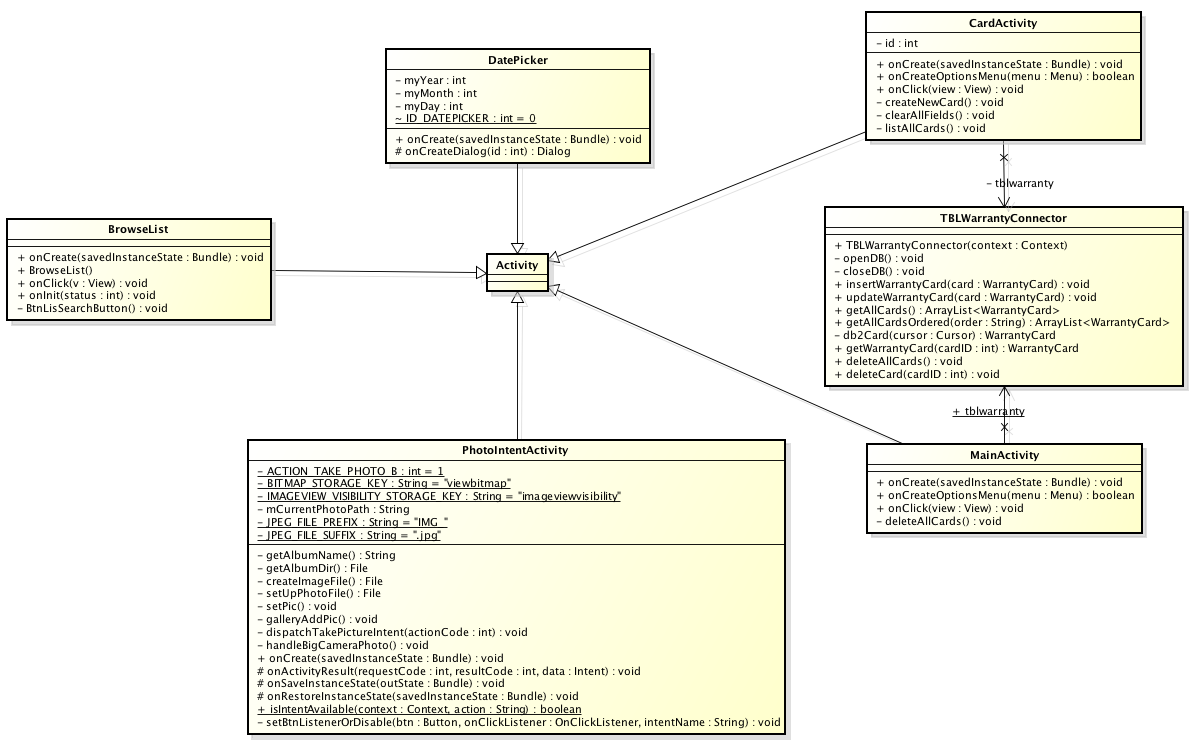
\includegraphics[width=\textwidth]{class_diagramm_activity.png} 
\caption{Klassendiagramm Activity}
\end{figure}

Weiter Klassendiagramme befinden sich im Anhang (\ref{fig:Klassendiagramm_global} und \ref{fig:Klassendiagramm_2})